% !TEX root = /Users/kquine/Dropbox/Research/Papers/2015/CPS-SMT-RTSS/cps-rtss.tex

\section{Hybrid PALS}
\label{sec:hybrid-pals}


%\textbf{(Peter) Some very important overview text added!}

This section presents \emph{Hybrid PALS}, which extends PALS to hybrid
systems.  One main difference between PALS and Hybrid PALS is that
 the time at which an event takes place does not matter in PALS, as
long as it happens within a certain time interval. This
 allows us to relate a distributed
real-time system to an essentially untimed synchronous model. However,
in hybrid systems, we cannot abstract from the time at which a
continuous value is read or  an actuator command is given
(both of which depend on a node's imprecise local clocks). Therefore,
the precise times at which these events happen must be included also
in the \emph{synchronous} Hybrid PALS models to have any possibility
of a bisimulation between the synchronous model and the distributed
hybrid system. 


In Hybrid PALS, a  state of a physical environment %of a machine $M$ 
is given by 
a tuple $\vec{v} = (v_1,\ldots,v_l) \in \mathbb{R}^l$ 
of its physical parameters $\vec{x} = (x_1, \ldots,x_l)$,
and
the behavior of %the physical parameters 
$\vec{x}$
can be modeled using ODEs that specify \emph{trajectories} 
$\tau_1, \ldots, \tau_l$ of %the parameters 
$\vec{x}$ over time.
%
%The continuous dynamics %of the system 
%is specified by \emph{controlled physical environments} $E$.
The standard PALS models $\mathcal{E}$ and $\mathcal{MA}(\mathcal{E},T,\Gamma)$ 
are  nondeterministic models defined for \emph{any possible} environment behaviors.
Then,
the \emph{environment restrictions} 
$\mathcal{E} \restriction E$ and
$\mathcal{MA}(\mathcal{E},T,\Gamma)\restriction E$
%introduced in~\cite{hybrid-pals}, 
 define the behavior of the models 
 constrained by the physical  environment $E$.  To have any
 control over when values are read from, and sent to, physical environments, we add in this paper \emph{sampling and
   response timing policies} to the Hybrid PALS models. 
We then  
prove a bisimulation equivalence 
relating $\mathcal{E}\restriction E$ and $\mathcal{MA}(\mathcal{E}, T,\Gamma)\restriction E$,
%with respect to physical environments,
which generalizes the  trace equivalence result in \cite{hybrid-pals}.



\subsection{Controlled Physical Environments}

%Let $\vec{\tau}(t) = (\tau_1(t),\ldots,\tau_l(t))$
%for an l-tuple of trajectories 
%$\vec{\tau} = (\tau_1,\ldots,\tau_l)$.
%Notice that the parameters $\vec{x}$ are also trajectories
%in such a way that a state of  the physical environment at time $t$


A (local)  physical environment $E_M$ of machine $M$
is specified as a   \emph{controlled physical environment}
that defines every possible trajectory of its physical parameters $\vec{x}$
for the control commands from $M$.
%
For a state $\vec{v} \in \mathbb{R}^l$, a control command $a$, and a duration $t \in \mathbb{R}$,
a controlled physical environment $E_M$
gives a trajectory $\vec{\tau}$ of its parameters $\vec{x}$ of duration $t$,
as illustrated in Fig.~\ref{fig:physical-transition}
%(e.g., state $v_1$, command $a$, duration $t_2-t_1$ yields trajectory $\tau_1$).

\begin{definition}
Let  $\mathcal{T}$ denote the set of all
trajectories (a trajectory of duration $T$ is a function $\tau : [0,T] \rightarrow \mathbb{R}$).
A \emph{controlled physical environment} $E_M = (C, \vec{x}, \Lambda)$ consists of:
\begin{inparaenum}[(i)]
    \item $C$ a set of \emph{control commands}; %(or ``actuator outputs'') from  $M$;
    \item $\vec{x} = (x_1, \ldots,x_l)$ a vector of real number variables; and
    \item $\Lambda \subseteq (C \times \mathbb{R}_{\geq 0} \times \mathbb{R}^l) \times \mathcal{T}^l$
    a \emph{physical transition relation}, where
    $((a, t, \vec{v}),  \vec{\tau}) \in \Lambda$
    iff for a control command $a \in C$ that lasts 
    for duration~$t$, 
    $E_M$'s physical state $\vec{x}$ follows the trajectory 
    $\vec{\tau} \in \mathcal{T}^l$
    from $\vec{v} \in \mathbb{R}^l$ with
        $\vec{\tau}(0) = \vec{v}$.
\end{inparaenum}
(E.g., $((a_1,t_2-t_1,v_1), \tau_1) \in \Lambda$ in Fig.~\ref{fig:physical-transition}).
\end{definition}

\begin{figure}
\centering
\begin{tikzpicture}[xscale=2.5,yscale=2.12,font=\footnotesize]
%baseline
\draw[-latex,thin] (-0.1,0) -- (3.2,0);
\draw[shift={(0,0)},thin,dashed] (0,1.1) -- (0,-0.05) node[below] {\footnotesize $t_0$};
\draw[shift={(0.7,0)},thin,dashed] (0,1.1) -- (0,-0.05) node[below] {\footnotesize $t_1$};
\draw[shift={(2.1,0)},thin,dashed] (0,1.1) -- (0,-0.05) node[below] {\footnotesize $t_2$};
\draw[shift={(3,0)},thin,dashed] (0,1.1) -- (0,-0.05) node[below] {\footnotesize $t_3$};
%curves
\begin{scope}[yshift=6pt]
\filldraw (0,0.21) circle (0.5pt) node[below,xshift=-1.2ex] {$v_0$};
\draw (0,0.21) .. controls (0.3,0.15) and (0.4,0.5) .. node[above,sloped] (t0) {$\tau_0$} (0.7,0.35);
\draw[-open triangle 45,very thin] ($(t0.north) + (-0.1,0.15)$) node[above] {$a_0$} -- ($(t0.north) + (-0.02,0.02)$);
    \filldraw (0.7,0.35) circle (0.5pt) node[below,xshift=-1.2ex] {$v_1$};
    \draw (0.7,0.35) .. controls (1.3,0.25) and (1.6,0.4) .. node[above,sloped] (t1) {$\tau_1$} (2.1,0.6);
    \draw[-open triangle 45,very thin] ($(t1.north) + (-0.2,0.15)$) node[left,yshift=2pt] {$a_1$} -- ($(t1.north) + (-0.02,0.02)$);
	\filldraw (2.1,0.6) circle (0.5pt) node[above,xshift=-1.2ex] {$v_2$};
	\draw (2.1,0.6) .. controls (2.6,0.7) and (2.7,0.7) .. node[above,sloped] (t2) {$\tau_2$} (3,0.77);
	\draw[-open triangle 45,very thin] ($(t2.west) + (-0.15,0.05)$) node[left,yshift=1pt] {$a_2$} -- ($(t2.west) + (-0.02,0.01)$);
	    \filldraw (3,0.77) circle (0.5pt) node[right,yshift=1ex] {$v_3$};
	\draw (2.1,0.6) .. controls (2.6,0.7) and (2.7,0.4) .. node[below,sloped] (t2') {$\tau_2'$} (3,0.57);
	    \filldraw (3,0.57) circle (0.5pt) node[right,yshift=-0.2ex] {$v_3'$};
	\draw[-open triangle 45,very thin] ($(t2'.west) + (-0.15,-0.1)$) node[left,yshift=-1pt] {$a_2'$} -- ($(t2'.west) + (-0.02,-0.02)$);

    \draw (0.7,0.35) .. controls (1.3,0.15) and (1.6,0.5) .. node[below,sloped] (t1') {$\tau_1'$} (2.1,0.1);
    \draw[-open triangle 45,very thin] ($(t1'.south) + (-0.2,-0.15)$) node[left,yshift=-2pt] {$a_1'$} -- ($(t1'.south) + (-0.02,-0.02)$);
	\filldraw (2.1,0.1) circle (0.5pt) node[below,xshift=-1.5ex] {$v_2'$};
	\draw (2.1,0.1) .. controls (2.6,-0.1) and (2.7,0.3) .. node[below,sloped] (t2''){$\tau_2''$} (3,0.2);
	\draw[-open triangle 45,very thin] ($(t2''.west) + (-0.15,-0.05)$) node[left,yshift=-1pt] {$a_2''$} -- ($(t2''.west) + (-0.02,-0.02)$);
	    \filldraw (3,0.2) circle (0.5pt) node[right,yshift=-1.5ex] {$v_3''$};;;
\end{scope}
\end{tikzpicture}
\caption{A controlled physical environment $E_M$.}
\label{fig:physical-transition}
\end{figure}


Several physical environments may be physically correlated,
and one %local 
environment may % immediately
affect  another environment.
Such %physical 
correlations are %naturally 
expressed as
\emph{time-invariant constraints} $(\forall t.\, \psi)$ of physical parameters over time $t$.
%(e.g., some parameter of one physical environment should always 
%  equal some other  parameter of another physical environment).
For example, if %physical 
parameter $x_1$ of $E_{M_1}$
must be equal to  parameter $x_2$ of %another environment 
$E_{M_2}$,
then the time-invariant constraint is  %the formula
$\forall t.\; x_1(t) = x_2(t)$.
%\footnote{Without loss of generality, we assume that different parameter names of different components are all different.}
%with variable $t$ for time.




\subsection{Environment-Restricted Controllers}
\label{sec:env-res}

A controller $M$ is a \emph{nondeterministic} machine
parameterized by any behavior of its %physical 
environment $E_M$.
%
The controller 
$M$ interacts  with %its physical environment 
$E_M$
according to its local clock,
which may  differ from global time by up to  
the maximal clock skew $\epsilon$.
Let $c_M : \mathbb{N} \to \mathbb{R}_{>0}$ denote a a \emph{periodic local clock} of $M$
that gives the \emph{global time} at the
beginning of the $(i+1)$-th period according to $M$'s local clock. 
That is,  $c_M(0) = 0$
and
$c_M(n) \in (n T - \epsilon, n T + \epsilon)$ for each $n > 0$.



\begin{figure}
\centering
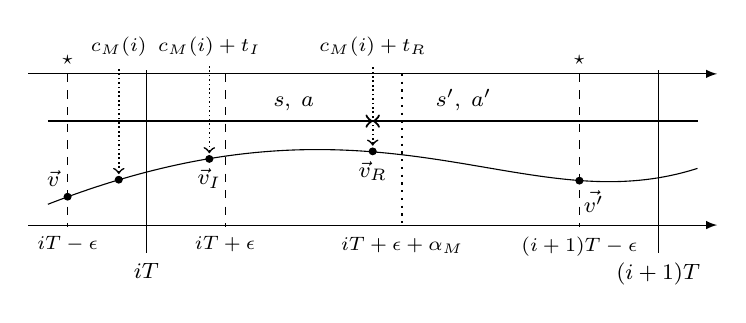
\begin{tikzpicture}[xscale=2.5,yscale=2.4,font=\footnotesize]
%baseline
\draw[-latex,thin] (-0.2,0) -- (3.3,0);
\draw[-latex,thin] (-0.2,0.8) -- (3.3,0.8);

\draw[thin] (0.4,0.82) -- (0.4,-0.15) node[below] { $iT$};
\draw[thin] (3,0.82) -- (3,-0.15) node[below] { $(i+1)T$};

\draw[->,thick] (-0.1,0.55) -- node[above,xshift=7ex] {$s,\; a$} (1.55,0.55);
\draw[<-,thick] (1.55,0.55) -- node[above,xshift=-6ex] {$s',\; a'$} (3.2,0.55);

\begin{scope}[font=\scriptsize]
\draw[dashed] (0,0.8) node[above] {$\star$} -- (0,-0.01) node[below] {$iT - \epsilon$} ;
\draw[dashed] (0.8,0.8) -- (0.8,-0.01) node[below] {$iT + \epsilon$};
\draw[dotted,thick] (1.7,0.8) -- (1.7,-0.01) node[below] {$iT + \epsilon + \alpha_M$};
\draw[dashed] (2.6,0.8) node[above] {$\star$}  -- (2.6,-0.01) node[below] { $(i+1)T - \epsilon$};

\draw[<-,densely dotted,semithick] (0.26,0.27) -- (0.26,0.84) node[above] {$c_M(i)$};
\draw[<-,densely dotted,semithick] (0.72,0.38) -- (0.72,0.84) node[above] {$c_M(i) + t_I$};
\draw[<-,densely dotted,semithick] (1.55,0.42) -- (1.55,0.84) node[above] {$c_M(i) + t_R$};
\end{scope}

\filldraw (0,0.15) circle (0.5pt) node[above,xshift=-1.2ex] {$\vec{v}$};
\filldraw (0.26,0.24) circle (0.5pt);
\filldraw (0.72,0.35) circle (0.5pt) node[below] {$\vec{v}_I$};
\filldraw (1.55,0.39) circle (0.5pt) node[below] {$\vec{v}_R$};
\filldraw (2.6,0.235) circle (0.5pt) node[below,xshift=1.2ex] {$\vec{v'}$};
\draw (-0.1,0.11) .. controls (1.6,0.8) and (2.3,0.0) .. (3.2,0.3);
\end{tikzpicture}
\caption{Timeline for an environment-restricted controller $M \restriction E_M$
with a local clock $c_M$, an environment sampling time $t_I$, and an response time $t_R$.}
\label{fig:env-restriction}
\end{figure}



Fig.~\ref{fig:env-restriction} depicts the behavior of 
the \emph{environment restriction} $M \restriction E_M$ %of  $M$ by   $E_M$ 
in a PALS distributed model. % $\mathcal{MA}(\mathcal{E},T,\Gamma)$.
Its $(i+1)$-th period begins  at time $c_M(i) \in (i T - \epsilon, i T + \epsilon)$. 
% according to its local clock $c_M$.
As explained in Section~\ref{pals-dist}, $M$ has already received all the inputs $\vec{i}$ %for this round 
before time $i T - \epsilon$.  At this time, $M$ also samples the
appropriate values of its environment $E_M$. The sampling takes time
$t_I$, so that 
the physical state $\vec{v}_I$ of $E_M$ is read at time $c_M(i) + t_I$.
$M$ executes its transition based on the inputs $\vec{i}$, the %sampled 
physical state $\vec{v}_I$,  and the current 
machine state $s$.
%
After the execution ends,
the machine state changes to  $s'$, and the new controller command $a$
is sent to $E_M$  at time  $c_M(i) + t_R$, %where it is treated immediately.
where $t_R$ denotes the response time, 
which equals the transition execution time and the actuator processing time.
The new outputs $\vec{o}$ from $M$ are delivered to their destination before $(i+1) T - \epsilon$.
%footnote{KYUNGMIN:  this last sentence is my understanding; is it correct?  We need to
%  explain clearly exactly when sampling and actuating take place, and  that's what I have tried.}




%We assume that 
A control command from a controller $M$ depends on $M$'s current 
machine state.
In Fig.~\ref{fig:env-restriction}, a current control command $a$ (given by $s$) remains effective 
until the execution ends at time $c_M(i) + t_R$,
and then a new control command $a'$ (given by $s'$) takes effect.
A physical environment 
$E_M$ defines trajectories of its parameters $\vec{x}$:
\begin{inparaenum}[(i)]
    \item from state $\vec{v}$ to $\vec{v}_I$ for the interval $[iT - \epsilon, c_M(i) + t_I]$ by the current command $a$,
    \item from $\vec{v}_I$ to $\vec{v}_R$ for the interval $[c_M(i) + t_I, c_M(i) + t_R]$ by again $a$, and 
    \item from $\vec{v}_R$ to $\vec{v'}$ for $[c_M(i) + t_R, (i+1)T-\epsilon]$ by the new control command $a'$.
\end{inparaenum}
Notice that $0 \leq t_I \leq t_R \leq \alpha_M$ for the maximal execution time $\alpha_M$  of $M$.
As a result,
a \emph{big step} transition of $M \restriction E_M$ from state $(s, \vec{v})$ with input $\vec{i}$ 
to state $(s',\vec{v'})$ with output $\vec{o}$
is defined for the time interval $[iT - \epsilon, (i+1)T-\epsilon]$ in \emph{distributed PALS models}.

% Moreover, $M \restriction E_M$ 
% can be considered as a ``normal'' state machine
% in \emph{synchronous models},
% provided that the timing values (such as $c_M(i)$, $t_I$, and $t_R$)
% as well as control commands are  determined by $M$'s machine states
% and inputs.\footnote{KYUNGMIN:  This last paragraph seems a little
%   unmotivated and misplaced here; can it be dropped?  Instead, it
%   would be MUCH better to informally introduce ``interfaces'' before
%   giving the definition ...}

A machine $M$ that integrates both a controller and its environment
should have a state space of the form $S\times \mathbb{R}^m$,  where
$\mathbb{R}^m$ is the state space of the $m$ physical parameters that
$M$ observes.   That $M$ has a transition for \emph{any} environment
values follows directly from the definitions of machines: their
transition relations are total. To compose such a machine with its
environment, we must define the ``interface'' between the controller
part and the ``environment part'' of such an environment-parametric
machine $M$. This interface is given by the following projection functions:


\begin{definition}
\label{def:env-interface}
% Suppose that $M$ has a state space of the form
% $S\times \mathbb{R}^m$  for $\mathbb{R}^m$ the $m$ physical parameters that $M$ observes.   
% For $(s,\vec{v}_o) \in S \times \mathbb{R}^m$,
The \emph{interface} of a controller $M$ is given by the %following
projection functions $\pi=(\pi_T, \pi_R, \pi_I, \pi_C, \pi_O)$, where $s\in S$ is a state in $M$: 
\begin{inparaenum}[(i)]
        \item $\pi_T(s) \in \mathbb{N}$ a ``round'' number; 
        %(i.e., $\pi_T(s) = i$ means that the next iteration of the system is iteration $i$); 
        \item $\pi_R(s,\vec{i}) \in \mathbb{R}$ a %environment 
        response time;
        \item $\pi_I(s) \in \mathbb{R}$ a %environment 
        sampling time;
        and    
        \item $\pi_C(s) \in C$ the control command of $M$  to $E_M$.
\end{inparaenum}
For state $\vec{v} \in \mathbb{R}^l$ of $E_M$,  
the \emph{observable} part of $\vec{v}$ by $M$
is given by the projection function 
$\pi_O(\vec{v}) \in \mathbb{R}^{m}$.
\end{definition}

The environment restriction of $M$ can then be defined in the expected way:
% Given state $(s, \vec{v})$ and input $\vec{i}$,
% the next state $(s', \vec{v'})$ and output $\vec{o}$ can be constructed %using $M$ and $E_M$
% by the same process of Fig.~\ref{fig:env-restriction}:

\begin{definition}
\label{def:env-res}
The \emph{environment restriction} of $M$ by $E_M$ 
with an interface $\pi$ is %the machine
$M \restriction_\pi E_M = (D_i, S \times \mathbb{R}^l, D_o, \delta_{M \restriction_\pi E_M})$,
where
$( (\vec{i}, (s,\vec{v})), ((s',\vec{v'}), \vec{o}) ) \in \delta_{M \restriction_\pi E_M}$ holds iff
 $\pi_T(s') = i + 1$ for the round number $i = \pi_T(s)$, and:
\begin{enumerate}
    \item %(Sampling) 
    $((a,u_I,\vec{v}),\tau_I) \in \Lambda$ and $\vec{v}_I = \tau_I(u_I)$,
    for  $t_I = \pi_I(s)$, duration $u_I = (c_M(i)+t_I)-(iT-\epsilon)$, and
    the current controller command $a = \pi_C(s)$;

    \item %(Execution) 
    $((a,u_R-u_I,\vec{v}_I),\tau_R) \in \Lambda$ and $\vec{v}_R = \tau_R(u_R-u_I)$,
    for $t_R = \pi_R(s,\vec{i})$ and $u_R = (c_M(i)+t_R) - (iT-\epsilon)$;

    \item %(Transition) 
    $( (\vec{i}, (s,\pi_O(\vec{v}_I))), ((s',\pi_O(\vec{v'})), \vec{o}) ) \in \delta_{M}$; and
    
    \item %(Waiting) 
    $((a',T - u_R,\vec{v}_R),\tau_W) \in \Lambda$ and  $\vec{v'} = \tau_W(T - u_R)$,
    for the next control command $a' = \pi_C(s')$.
\end{enumerate}
\end{definition}



\subsection{Hybrid PALS}

Hybrid PALS models are parameterized by \emph{sampling and response timing policies}
that 
determine sensor sampling timing $t_I$ and actuator response timing $t_R$.
%besides  bounds $\Gamma$.
Such a policy 
is given as a collection of 
projection functions $\pi=(\pi_T, \pi_R, \pi_I, \pi_C, \pi_O)$ 
in Definition~\ref{def:env-interface}.
The continuous dynamics %of a PALS system 
is ``completely'' decided  
by the controllers % (in $\mathcal{E}$ or $\mathcal{MA}(\mathcal{E},T,\Gamma)$),
their physical environments, and timing policies (including local clocks of controllers). 
%  \textbf{(Peter)  Are the clock functions also parameters, or are we quantifying over
%  all local clock skews??}


Deciding $\pi$ is a design choice. 
% Most generally, values of $\pi$ can vary
% according to states and inputs.
% More realistically, sampling/response timings are fixed 
% to certain numbers to simplify the system complicity.
In % our previous work
\cite{hybrid-pals}, $t_I$ is $0$ 
(for controllers tightly integrated with its environments)
and $t_R$ is  
the maximum execution time $\alpha_{\max}$.


The synchronous model in Hybrid PALS is specified
as a multirate ensemble $\mathcal{E}$ and  the physical environments of subcomponents,
where physical correlations between those environments
are specified as time-invariant constraints.

\begin{definition}
A \emph{hybrid multirate ensemble} $\mathcal{E}\restriction_{\Pi} E_{\mathcal{E}}$
is given by:
\begin{inparaenum}[(i)]
    \item a multirate ensemble $\mathcal{E}$, %= (J_S ,  J_F, e, \{M_j\}_{j\in J_S \cup J_F}, E, \mathit{src}, \mathit{rate}, \mathit{adap})$ 
    \item a family of policy functions $\Pi=\{\pi_j\}_{j\in J_S  \cup J_F}$
    (with $J_S$ an index set of slow machines and $J_F$ an index set of fast machines),
    and
    \item a family of local physical environments 
    $E_\mathcal{E} = \langle\{E_{M_j}\}_{j\in J_S \cup J_F}, \forall t.\, \psi)\rangle$ 
    with $\forall t.\,\psi$ the time-invariant constraints.
\end{inparaenum}
\end{definition}   


The behaviors of a hybrid ensemble  $\mathcal{E} \restriction_{\Pi} E_\mathcal{E}$
are  a \emph{subset} of the behaviors of $\mathcal{E}$, namely, the behaviors restricted by 
the physical environment $E_\mathcal{E}$.
As mentioned,
each (decelerated) environment-restricted machine $M_j \restriction_\pi E_{M_j}$ defines 
a transition from a state  at time $iT - \epsilon$ to one at time $(i+1)T-\epsilon$ for a global period $T$.
Therefore, a lock-step composition of such %environment-restricted 
transitions
\emph{that also satisfy the time-invariant constraints} gives a transition of 
the synchronous composition $M_{\mathcal{E} \restriction_{\Pi} E_\mathcal{E}}$
from one state at time $iT - \epsilon$ to another state at time $(i+1)T-\epsilon$.


Hybrid PALS maps a hybrid multirate ensemble
$\mathcal{E}\restriction_{\Pi} E_\mathcal{E}$ with a global period $T$, 
together with PALS bounds $\Gamma$,  to the distributed hybrid system  
$\mathcal{MA}(\mathcal{E}, T, \Gamma) \restriction_{\Pi} E_\mathcal{E}$.
Similarly, its  behaviors are the subset of those of the %PALS
distributed system $\mathcal{MA}(\mathcal{E}, T, \Gamma)$ that can be realized
by the %physical 
environment $E_\mathcal{E}$
and satisfy the time-invariant constraints.
In particular, big-step transitions of each component $M_j \restriction_\pi E_{M_j}$ are
defined for the interval $[iT - \epsilon, (i+1)T-\epsilon]$
 as explained in Section~\ref{sec:env-res}.


The correctness of Hybrid PALS follows from the fact that 
all physical measurements and physical activation \emph{happen at the same time}
in both $\mathcal{E} \restriction_{\Pi} E_\mathcal{E}$  and $\mathcal{MA}(\mathcal{E}, T, \Gamma) \restriction_{\Pi} E_\mathcal{E}$ with the \emph{same timing policies} $\Pi$.
%(see Definition~\ref{def:env-res}).
%
Recall that stable states of $\mathcal{MA}(\mathcal{E}, T, \Gamma)$ are states at times $iT - \epsilon$.
Hence,  big-step ``stable'' transitions are well defined for 
$\mathcal{MA}(\mathcal{E}, T, \Gamma) \restriction_{\Pi} E_\mathcal{E}$
from $iT - \epsilon$ to $(i+1)T-\epsilon$,
which are exactly related to single steps of the synchronous composition 
$M_{\mathcal{E} \restriction_{\Pi} E_\mathcal{E}}$ (by the same relation $(\sim_\mathit{obi} \,;\, \mathit{sync})$ in Theorem~\ref{thm:mr-pals}).
Consequently, we have:


\begin{theorem}\label{thm:hybrid-pals} 
The relation $(\sim_\mathit{obi} \,;\, \mathit{sync})$ 
is a bisimulation between 
the transition system by $\mathcal{E} \restriction_{\Pi} E_\mathcal{E}$ 
and the big-step stable transition system induced by $\mathcal{MA}(\mathcal{E}, T, \Gamma) \restriction_{\Pi} E_\mathcal{E}$.
\end{theorem}





